\section{Effect of $\hat{\pfrac}$ on contingency table entries and common performance metrics} \label{partial}
To study the effect of imprecise estimates of $\pfrac$, we start by computing partial derivatives of each entry of the partial contingency table based on unlabeled instances to $\hat{\pfrac}$ (see Section~\ref{contingency}). Subsequently, we will compute partial derivatives of TPR, FPR and precision to $\hat{\pfrac}$ to describe the effect of estimating $\pfrac$ on (area under) ROC and PR curves.

For ease of notation, we base all subsequent calculations on $\tilde{\theta} = \hat{\pfrac} \mathcal{T}(r) \cdot |\unlabeled| \approx \theta$ which ignores the discrete effect of rounding in the real definition of $\theta$ (Eq.~\ref{theta}). We additionally assume it is possible to assign the desired amount $\tilde{\theta}$ of surrogate positives in $\topfun(\unlabeled, r)$, which holds for ranks $r$ that are not too close to the top or bottom of $\overall$, given reasonable values of $\hat{\pfrac}$ and CDF bounds $\mathcal{T}(r)$.\footnote{$\mathcal{T}(r)$ represents a bound on rank CDF, that is either $\mathcal{T}_{lb}(r)$ or $\mathcal{T}_{ub}(r)$ as used in the manuscript.} If this does not hold, that is when there is clipping in Eq.~\ref{eq:surrpos-conditions}, then (small) changes in $\hat{\pfrac}$ do not affect $\TP_U^r$ and hence the partial derivatives of \emph{all} entries in the contingency table to $\hat{\pfrac}$ are effectively 0.

Given these simplifications, the partial contingency table based on unlabeled instances becomes:
\begin{align*}
\TP_U^r &= \tilde{\theta} = \hat{\pfrac}\mathcal{T}(r) \cdot |\unlabeled| \\
\FN_U^r &= |\surrpos| - \TP_U^r = \hat{\pfrac}\cdot |\unlabeled| - \hat{\pfrac}\mathcal{T}(r) \cdot |\unlabeled| = \hat{\pfrac} \big(1-\mathcal{T}(r)\big) \cdot|\unlabeled| \nonumber \\
\FP_U^r &= |\topfun(\unlabeled, r)| - \TP_U^r = |\topfun(\unlabeled, r)| - \hat{\pfrac}\mathcal{T}(r) \cdot |\unlabeled|, \nonumber \\
\TN_U^r &= |\unlabeled| - |\surrpos| - \FP_U^r = |\unlabeled| - \hat{\pfrac}\cdot|\unlabeled| - |\topfun(\unlabeled, r)| + \hat{\pfrac}\mathcal{T}(r) \cdot |\unlabeled|, \\
	&= \big(1-\hat{\pfrac} + \hat{\pfrac}\mathcal{T}(r)\big) \cdot |\unlabeled| - |\topfun(\unlabeled, r)|.
\end{align*}
The partial derivatives of each entry of the partial contingency table then become:
\begin{align*}
\frac{\partial \TP_U^r}{\partial \hat{\pfrac}} &= \mathcal{T}(r) \cdot |\unlabeled| \geq 0, & &\frac{\partial \FP_U^r}{\partial \hat{\pfrac}} = -\mathcal{T}(r) \cdot |\unlabeled| \leq 0, \\
\frac{\partial \FN_U^r}{\partial \hat{\pfrac}} &= \big(1 -\mathcal{T}(r)\big) \cdot |\unlabeled| \geq 0, & &\frac{\partial \TN_U^r}{\partial \hat{\pfrac}} = \big(\mathcal{T}(r)-1\big) \cdot |\unlabeled| \leq 0.
\end{align*}

Partial derivatives for TPR, TPR and precision are a little more involved:
\begin{align}
\frac{\partial \TPR_U^r}{\partial \hat{\pfrac}} &= \frac{\frac{\partial \TP_U^r}{\partial \hat{\pfrac}} |\surrpos| - \TP_U^r \frac{\partial |\surrpos|}{\partial \hat{\pfrac}}}{|\surrpos|^2} 
= \frac{\mathcal{T}(r)\hat{\pfrac}\cdot|\unlabeled|^2-\mathcal{T}(r)\hat{\pfrac} |\unlabeled|^2}{\hat{\pfrac}^2|\unlabeled|^2} \nonumber \\
&= \frac{\mathcal{T}(r)-\mathcal{T}(r)}{\hat{\pfrac}} = 0 \label{eq:dtpr} \\
\frac{\partial \FPR_U^r}{\partial \hat{\pfrac}} &= \frac{\frac{\partial \FP_U^r}{\partial \hat{\pfrac}} \cdot (|\unlabeled|-|\surrpos|) - \FP_U^r \frac{\partial (|\unlabeled|-|\surrpos|)}{\partial \hat{\pfrac}}}{(|\unlabeled|-|\surrpos|)^2} \nonumber \\
&= \frac{-\mathcal{T}(r) \cdot |\unlabeled| \cdot (|\unlabeled|-|\surrpos|)+\FP_U^r \cdot |\unlabeled|}{(|\unlabeled|-|\surrpos|)^2} \nonumber \\
&=\frac{-\mathcal{T}(r) (1-\hat{\pfrac}) \cdot |\unlabeled|^2 + \FP_U^r \cdot |\unlabeled|}{(1-\hat{\pfrac})^2 \cdot |\unlabeled|^2} \nonumber \\
&=\frac{-\mathcal{T}(r)}{1-\hat{\pfrac}} + \frac{(|\topfun(\unlabeled, r)|-\hat{\pfrac}\mathcal{T}(r) \cdot |\unlabeled|) \cdot |\unlabeled|}{(1-\hat{\pfrac})^2 \cdot |\unlabeled|^2}  \nonumber \\
%&=\frac{-\mathcal{T}(r)}{1-\hat{\pfrac}} - \frapfrac}\mathcal{T}(r)}{(1-\hat{\pfrac})^2} + \frac{|\topfun(\unlabeled, r)|}{(1-\hat{\pfrac})^2\cdot|\unlabeled|} 
&=\frac{-\mathcal{T}(r)}{(1-\hat{\pfrac})^2} + \frac{|\topfun(\unlabeled, r)|}{(1-\hat{\pfrac})^2\cdot|\unlabeled|} 
= \frac{|\topfun(\unlabeled, r)| - \mathcal{T}(r) \cdot |\unlabeled|}{(1-\hat{\pfrac})^2} \label{eq:dfpr} \\
%=\frac{-\mathcal{T}(r)}{(1-\hat{\pfrac})^2} + \frac{|\topfun(\unlabeled, r)|}{(1-\hat{\pfrac})^2\cdot|\unlabeled|} \nonumber \\
%&= \frac{|\topfun(\unlabeled, r)| - \mathcal{T}(r) \cdot |\unlabeled|}{(1-\hat{\pfrac})^2} \label{eq:dfpr} \\
\frac{\partial \PREC_U^r}{\partial \hat{\pfrac}} &= \frac{\frac{\partial \TP_U^r}{\partial \hat{\pfrac}} \cdot (\TP_U^r+\FP_U^r) - \TP_U^r \frac{\partial (\TP_U^r+\FP_U^r)}{\partial \hat{\pfrac}}}{(\TP_U^r+\FP_U^r)^2} \nonumber \\ 
&= \frac{\mathcal{T}(r)\cdot|\unlabeled|\cdot(\TP_U^r + \FP_U^r)}{(\TP_U^r + \FP_U^r)^2} \nonumber \\
&= \frac{\mathcal{T}(r)\cdot|\unlabeled|}{(\TP_U^r + \FP_U^r)} = \frac{\mathcal{T}(r)\cdot|\unlabeled|}{|\topfun(\unlabeled,r)|} \geq 0 \label{eq:dprec} 
\end{align}
%$\partial \FPR_U^r / \partial \hat{\pfrac}$ is particularly interesting: it is positive if the ranking is better than random, i.e. $\TPR(\surrpos, r) > \FPR(\surrpos, r)$ and negative when the ranking is worse than random, i.e. $\TPR(\surrpos, r) < \FPR(\surrpos, r)$. This was already shown previously in Lemma~\ref{lemma-size-fpr}. 

Both $\partial \FPR_U^r / \partial \hat{\pfrac}$ and $\partial \PREC_U^r / \partial \hat{\pfrac}$ are a function of $\mathcal{T}(r)$, while $\partial \FPR_U^r / \partial \hat{\pfrac} = 0$. This implies that the ordering of rankings in terms of area under the ROC curve can change when the estimate of $\pfrac$ changes, as proven by example in Figure~\ref{rocauc-switch}.


\section{The effect of the fraction of known positives, known negatives and $\hat{\pfrac}$} \label{knownneg}
Known negatives can be incorporated in our approach as described in Section~\ref{contingency}. Given a fixed ranking $\overall$, having known negatives essentially reduces the size of the unlabeled subset $\unlabeled$, which in turn reduces the number of degrees of freedom in assigning surrogate positives. As such, known negatives provide some benefit, though this is small in practice. Table~\ref{parameffects-posonly} illustrates the effect of increasing amounts of known positives and known negatives: known positives significantly tighten bounds on AUROC, while known negatives only do so marginally (cfr. bounds with $10\%$ known positives and $40/60/80\%$ known negatives).

\def\realauc{0.765}

\newcommand{\plotauc}[2]{
\begin{tikzpicture}[baseline=1ex]
    \begin{axis}[hide axis,clip=false,
%	xmin=0.71,xmax=0.84,xlabel={X},
%	ymin=-1,ymax=1,
%	x=20cm, y=0.8em,
	xmin=0.67,xmax=0.87,xlabel={X},
	ymin=-1,ymax=1,
	x=12cm, y=0.8em,
	]

\addplot[black, very thick, dashed] coordinates {(\realauc, -1) (\realauc, 1)};
\addplot[gray, thick, dashed] coordinates {(0.67, -1) (0.67, 1)};
\addplot[gray, thick, dashed] coordinates {(0.87, -1) (0.87, 1)};
%\addplot[gray, thick, dashed] coordinates {(0.71, -1) (0.71, 1)};
%\addplot[gray, thick, dashed] coordinates {(0.83, -1) (0.83, 1)};
\addplot[black, dotted] coordinates {(0.73, -1) (0.73, 1)};
\addplot[black, dotted] coordinates {(0.75, -1) (0.75, 1)};
\addplot[black, dotted] coordinates {(0.77, -1) (0.77, 1)};
\addplot[black, dotted] coordinates {(0.79, -1) (0.79, 1)};
\addplot[black, dotted] coordinates {(0.81, -1) (0.81, 1)};
\addplot[gray, dotted] coordinates {(0.71, -1) (0.71, 1)};
\addplot[gray, dotted] coordinates {(0.69, -1) (0.69, 1)};
\addplot[gray, dotted] coordinates {(0.83, -1) (0.83, 1)};
\addplot[gray, dotted] coordinates {(0.85, -1) (0.85, 1)};
\draw [color=cyan!80!black, opacity=0.8] (axis cs: #1, -0.7) rectangle (axis cs: #2, 0.6);
\fill [color=cyan!80!black, opacity=0.4, fill] (axis cs: #1, -0.7) rectangle (axis cs: #2, 0.6);
    \end{axis}
\end{tikzpicture}
}
\newcommand{\plotauccolor}[3]{
\begin{tikzpicture}[baseline=1ex]
    \begin{axis}[hide axis,clip=false,
	xmin=0.67,xmax=0.87,xlabel={X},
	ymin=-1,ymax=1,
	x=12cm, y=0.8em,
	]

\addplot[black, very thick, dashed] coordinates {(\realauc, -1) (\realauc, 1)};
\addplot[gray, thick, dashed] coordinates {(0.67, -1) (0.67, 1)};
\addplot[gray, thick, dashed] coordinates {(0.87, -1) (0.87, 1)};
\addplot[black, dotted] coordinates {(0.73, -1) (0.73, 1)};
\addplot[black, dotted] coordinates {(0.75, -1) (0.75, 1)};
\addplot[black, dotted] coordinates {(0.77, -1) (0.77, 1)};
\addplot[black, dotted] coordinates {(0.79, -1) (0.79, 1)};
\addplot[black, dotted] coordinates {(0.81, -1) (0.81, 1)};
\addplot[gray, dotted] coordinates {(0.71, -1) (0.71, 1)};
\addplot[gray, dotted] coordinates {(0.69, -1) (0.69, 1)};
\addplot[gray, dotted] coordinates {(0.83, -1) (0.83, 1)};
\addplot[gray, dotted] coordinates {(0.85, -1) (0.85, 1)};
\draw [color=#3!80!black, opacity=0.8] (axis cs: #1, -0.7) rectangle (axis cs: #2, 0.6);
\fill [color=#3!80!black, opacity=0.4, fill] (axis cs: #1, -0.7) rectangle (axis cs: #2, 0.6);
    \end{axis}
\end{tikzpicture}
}
\newcommand{\plotauclabels}{
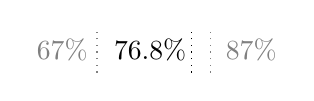
\begin{tikzpicture}[baseline=0.8ex]
    \begin{axis}[hide axis,clip=false,
	xmin=0.67,xmax=0.87,xlabel={X},
	ymin=-1,ymax=1,
	x=12cm, y=0.8em,
	]
\node [gray] at (axis cs: 0.67, 0) {$67\%$};
\node [black] at (axis cs: 0.763, 0) {$76.8\%$};
\node [gray] at (axis cs: 0.87, 0) {$87\%$};
\addplot[gray, dotted] coordinates {(0.7068, -1) (0.7068, 1)};
\addplot[gray, dotted] coordinates {(0.8268, -1) (0.8268, 1)};
\addplot[black, dotted] coordinates {(0.8068, -1) (0.8068, 1)};
    \end{axis}
\end{tikzpicture}
}


%\renewcommand{\arraystretch}{1.5}

However, when the number of known negatives is large, it may be useful to reverse our approach, i.e., start from the rank distribution of known negatives. To do so, we can essentially flip all known class labels, use $\bar{\pfrac}=1-\pfrac$ and adjust the resulting contingency tables accordingly.%, that is make the following changes: $\TP \rightarrow \FP$, $\FP\rightarrow\TP$, $\TN\rightarrow\FN$ and $\FN\rightarrow\TN$. 

Table~\ref{parameffects-both} shows bounds when based on known positives or known negatives (whichever are tightest). It is important to see that $|\knownneg| > |\knownpos|$ does not guarantee that performance bounds based on known negatives are tighter, because $\pfrac$ also affects the bounds. When computing performance bounds based on known negatives, overestimating $\hat{\pfrac}$ leads to underestimated bounds (since we use $\bar{\pfrac}=1-\hat{\pfrac}$) and vice versa. The effect of errors in $\hat{\pfrac}$ is opposite in bounds based on $\knownneg$.

Hence, bounds on performance metrics can be computed based primarily on known positives $\knownpos$ \emph{or} known negatives $\knownneg$. The width of the bounds depends on the combination of $|\knownpos|$ (or $|\knownneg|$) and $\pfrac$ (or $\bar{\pfrac}$) in a nontrivial way: depending on $\pfrac$, it is possible to obtain wider bounds based on known negatives, even if $|\knownneg| > |\knownpos|$ (or vice versa). In practice, we can estimate metrics based on $\knownpos$ and $\knownneg$ separately and then use whichever yields the tightest bounds, as shown in Table~\ref{parameffects-both}.

\begin{table}[!h]
\resizebox{\textwidth}{!}{
\begin{tabular}{ccccc|c|c}
\toprule
\multicolumn{3}{c}{configuration} & & \multicolumn{3}{c}{bounds on area under the ROC curve (true AUROC=$76.8\%$)} \\ \cline{1-3} \cline{5-7}
$\frac{|\knownpos|}{|\bothpos|}$	& $\frac{|\knownneg|}{|\mathcal{N}_\Omega|}$ & $\pfrac$ & & $\hat{\pfrac}\ /\ \pfrac = 0.8$ & $\hat{\pfrac}\ /\ \pfrac = 1.0$  & $\hat{\pfrac}\ /\ \pfrac = 1.2$ \\ 
\midrule
\ifdefined\showtikzplots
10				&	0	& 15	& & \plotauc{0.7099}{0.8063}  & \plotauc{0.7163}{0.8182}  & \plotauc{0.7235}{0.8303} \\
				&	20	& 18	& & \plotauc{0.7099}{0.8062}  & \plotauc{0.7163}{0.8180}  & \plotauc{0.7235}{0.8299} \\
				&	40	& 23	& & \plotauc{0.7099}{0.8060}  & \plotauc{0.7163}{0.8176}  & \plotauc{0.7235}{0.8289} \\
				&	60	& 31	& & \plotauc{0.7099}{0.8059}  & \plotauc{0.7163}{0.8059}  & \plotauc{0.7235}{0.8270} \\
				&	80	& 47	& & \plotauc{0.7099}{0.8055}  & \plotauc{0.7163}{0.8055}  & \plotauc{0.7235}{0.8160} \\
 & & & & \plotauclabels & \plotauclabels  & \plotauclabels \\
30				&	0	& 12	& & \plotauc{0.7328}{0.7732}  & \plotauc{0.7378}{0.7823}  & \plotauc{0.7434}{0.7915} \\
				&	20	& 15	& & \plotauc{0.7328}{0.7732}  & \plotauc{0.7378}{0.7823}  & \plotauc{0.7434}{0.7915} \\
				&	40	& 19	& & \plotauc{0.7328}{0.7732}  & \plotauc{0.7378}{0.7823}  & \plotauc{0.7434}{0.7914} \\
				&	60	& 26	& & \plotauc{0.7328}{0.7732}  & \plotauc{0.7378}{0.7823}  & \plotauc{0.7434}{0.7914} \\
				&	80	& 41	& & \plotauc{0.7328}{0.7732}  & \plotauc{0.7378}{0.7822}  & \plotauc{0.7434}{0.7907} \\
 & & & & \plotauclabels & \plotauclabels  & \plotauclabels \\
50				&	0	& 9	& & \plotauc{0.7455}{0.7682}  & \plotauc{0.7502}{0.7739}  & \plotauc{0.7573}{0.7807} \\
				&	20	& 11	& & \plotauc{0.7455}{0.7682}  & \plotauc{0.7542}{0.7779}  & \plotauc{0.7573}{0.7807} \\
				&	40	& 14	& & \plotauc{0.7455}{0.7682}  & \plotauc{0.7542}{0.7779}  & \plotauc{0.7573}{0.7807} \\
				&	60	& 20	& & \plotauc{0.7455}{0.7682}  & \plotauc{0.7542}{0.7779}  & \plotauc{0.7573}{0.7807} \\
				&	80	& 33	& & \plotauc{0.7455}{0.7682}  & \plotauc{0.7542}{0.7779}  & \plotauc{0.7573}{0.7804} \\
 & & & & \plotauclabels & \plotauclabels  & \plotauclabels \\
70				&	0	& 6	& & \plotauc{0.7533}{0.7646}  & \plotauc{0.7594}{0.7727}  & \plotauc{0.7676}{0.7778} \\
				&	20	& 7	& & \plotauc{0.7533}{0.7646}  & \plotauc{0.7594}{0.7727}  & \plotauc{0.7676}{0.7778} \\
				&	40	& 9	& & \plotauc{0.7533}{0.7646}  & \plotauc{0.7594}{0.7727}  & \plotauc{0.7676}{0.7778} \\
				&	60	& 13	& & \plotauc{0.7533}{0.7646}  & \plotauc{0.7594}{0.7727}  & \plotauc{0.7676}{0.7778} \\
				&	80	& 23	& & \plotauc{0.7533}{0.7646}  & \plotauc{0.7594}{0.7727}  & \plotauc{0.7676}{0.7778} \\
\fi
\bottomrule
\end{tabular}
}
\caption[]{Estimated bounds on AUROC under different configurations. The total data set comprises $2,000$ positives and $10,000$ negatives. We varied the fraction of known positives and known negatives, which also implies changing $\pfrac$. All entries in the table are in percentages. We used three estimates for $\hat{\pfrac}$, namely an underestimate, the correct value and an overestimate (left to right). \newline
Legend:
\begin{tikzpicture}[baseline=-0.5ex] \draw [color=black, thick, dashed] (0, 0) -- (0.5, 0); \end{tikzpicture} true AUROC, 

\begin{tikzpicture}[baseline=-0.5ex] \draw [color=cyan!80!black, opacity=0.8] (0, -0.15) rectangle (0.7, 0.25); 
\fill [color=cyan!80!black, opacity=0.4] (0, -0.15) rectangle (0.7, 0.25); \end{tikzpicture} bounds based on known positives.
}
\label{parameffects-posonly}
\end{table}


\begin{table}[!h]
\resizebox{\textwidth}{!}{
\begin{tabular}{ccccc|c|c}
\toprule
\multicolumn{3}{c}{configuration} & & \multicolumn{3}{c}{bounds on area under the ROC curve (true AUROC=$76.8\%$)} \\ \cline{1-3} \cline{5-7}
$\frac{|\knownpos|}{|\bothpos|}$	& $\frac{|\knownneg|}{|\mathcal{N}_\Omega|}$ & $\pfrac$ & & $\hat{\pfrac}\ /\ \pfrac = 0.8$ & $\hat{\pfrac}\ /\ \pfrac = 1.0$  & $\hat{\pfrac}\ /\ \pfrac = 1.2$ \\ 
\midrule
\ifdefined\showtikzplots
10 & 0 & 15 & & \plotauccolor{0.7081}{0.8044}{cyan} & \plotauccolor{0.7143}{0.8160}{cyan} & \plotauccolor{0.7214}{0.8277}{cyan} \\
 & 20 & 18 & & \plotauccolor{0.7081}{0.8043}{cyan} & \plotauccolor{0.7143}{0.8159}{cyan} & \plotauccolor{0.7214}{0.8274}{cyan} \\
 & 40 & 23 & & \plotauccolor{0.7950}{0.8724}{red} & \plotauccolor{0.7420}{0.8215}{red} & \plotauccolor{0.7067}{0.7742}{red} \\
 & 60 & 31 & & \plotauccolor{0.8106}{0.8531}{red} & \plotauccolor{0.7564}{0.8003}{red} & \plotauccolor{0.7182}{0.7538}{red} \\
 & 80 & 47 & & \plotauccolor{0.8072}{0.8287}{red} & \plotauccolor{0.7534}{0.7729}{red} & \plotauccolor{0.7165}{0.7301}{red} \\
 & & & & \plotauclabels & \plotauclabels  & \plotauclabels \\
30 & 0 & 12 & & \plotauccolor{0.7367}{0.7803}{cyan} & \plotauccolor{0.7417}{0.7896}{cyan} & \plotauccolor{0.7474}{0.7989}{cyan} \\
 & 20 & 14 & & \plotauccolor{0.7367}{0.7802}{cyan} & \plotauccolor{0.7417}{0.7896}{cyan} & \plotauccolor{0.7474}{0.7988}{cyan} \\
 & 40 & 18 & & \plotauccolor{0.7367}{0.7802}{cyan} & \plotauccolor{0.7417}{0.7895}{cyan} & \plotauccolor{0.7474}{0.7987}{cyan} \\
 & 60 & 25 & & \plotauccolor{0.7964}{0.8347}{red} & \plotauccolor{0.7567}{0.7996}{red} & \plotauccolor{0.7256}{0.7638}{red} \\
 & 80 & 41 & & \plotauccolor{0.7935}{0.8125}{red} & \plotauccolor{0.7539}{0.7727}{red} & \plotauccolor{0.7235}{0.7386}{red} \\
 & & & & \plotauclabels & \plotauclabels  & \plotauclabels \\
50 & 0 & 9 & & \plotauccolor{0.7488}{0.7706}{cyan} & \plotauccolor{0.7524}{0.7773}{cyan} & \plotauccolor{0.7564}{0.7841}{cyan} \\
 & 20 & 11 & & \plotauccolor{0.7488}{0.7706}{cyan} & \plotauccolor{0.7524}{0.7773}{cyan} & \plotauccolor{0.7564}{0.7841}{cyan} \\
 & 40 & 14 & & \plotauccolor{0.7488}{0.7706}{cyan} & \plotauccolor{0.7524}{0.7773}{cyan} & \plotauccolor{0.7564}{0.7840}{cyan} \\
 & 60 & 20 & & \plotauccolor{0.7488}{0.7706}{cyan} & \plotauccolor{0.7524}{0.7773}{cyan} & \plotauccolor{0.7564}{0.7840}{cyan} \\
 & 80 & 33 & & \plotauccolor{0.7807}{0.7992}{red} & \plotauccolor{0.7537}{0.7724}{red} & \plotauccolor{0.7313}{0.7475}{red} \\
 & & & & \plotauclabels & \plotauclabels  & \plotauclabels \\
70 & 0 & 5 & & \plotauccolor{0.7554}{0.7667}{cyan} & \plotauccolor{0.7576}{0.7709}{cyan} & \plotauccolor{0.7599}{0.7751}{cyan} \\
 & 20 & 6 & & \plotauccolor{0.7554}{0.7667}{cyan} & \plotauccolor{0.7576}{0.7709}{cyan} & \plotauccolor{0.7599}{0.7751}{cyan} \\
 & 40 & 9 & & \plotauccolor{0.7554}{0.7667}{cyan} & \plotauccolor{0.7576}{0.7709}{cyan} & \plotauccolor{0.7599}{0.7751}{cyan} \\
 & 60 & 13 & & \plotauccolor{0.7554}{0.7667}{cyan} & \plotauccolor{0.7576}{0.7709}{cyan} & \plotauccolor{0.7599}{0.7751}{cyan} \\
 & 80 & 23 & & \plotauccolor{0.7554}{0.7667}{cyan} & \plotauccolor{0.7576}{0.7709}{cyan} & \plotauccolor{0.7599}{0.7751}{cyan} \\
\fi
\bottomrule
\end{tabular}
}
\caption[]{Estimated bounds on AUROC under different configurations. The total data set comprises $2,000$ positives and $10,000$ negatives. We varied the fraction of known positives and known negatives, which also implies changing $\pfrac$. All entries in the table are in percentages. We used three estimates for $\hat{\pfrac}$, namely an underestimate, the correct value and an overestimate (left to right). In this table, we computed bounds based on known positives and known negatives (separately) and report the tightest confidence interval each time. \newline
Legend: 
\begin{tikzpicture}[baseline=-0.5ex] \draw [color=black, thick, dashed] (0, 0) -- (0.5, 0); \end{tikzpicture} true AUROC, bounds based on 

\begin{tikzpicture}[baseline=-0.5ex] \draw [color=cyan!80!black, opacity=0.8] (0, -0.15) rectangle (0.7, 0.25); 
\fill [color=cyan!80!black, opacity=0.4] (0, -0.15) rectangle (0.7, 0.25); \end{tikzpicture} known positives and 

\begin{tikzpicture}[baseline=-0.5ex] \draw [color=red!80!black, opacity=0.8] (0, -0.15) rectangle (0.7, 0.25); 
\fill [color=red!80!black, opacity=0.4] (0, -0.15) rectangle (0.7, 0.25); \end{tikzpicture} known negatives.}
\label{parameffects-both}
\end{table}
